\pagestyle{fancy}
\thispagestyle{fancy}
\chapter{Testing}
\section{Introduction to Testing}
Our testing strategy encompassed multiple layers of validation to ensure the reliability, security, and usability of the HealthHub platform. We implemented a comprehensive testing approach that covered both technical functionality and user experience.

\section{Types of testing done}
\subsection{Technical Testing}

\begin{enumerate}
    \item \textbf{Unit Testing}
    \begin{itemize}
        \item Frontend component testing using React Testing Library
        \item Backend API endpoint testing with pytest
        \item Database query validation
        \item AI model response validation
    \end{itemize}

    \item \textbf{Integration Testing}
    \begin{itemize}
        \item API integration tests
        \item Database interaction testing
        \item External service integration validation
        \item Sensor data processing verification
    \end{itemize}

    \item \textbf{Performance Testing}
    \begin{itemize}
        \item Load testing of API endpoints
        \item Database query optimization
        \item Real-time data processing efficiency
        \item Frontend rendering performance
    \end{itemize}
\end{enumerate}

\subsection{User Experience Testing}
\begin{figure}[H]
    \centering
    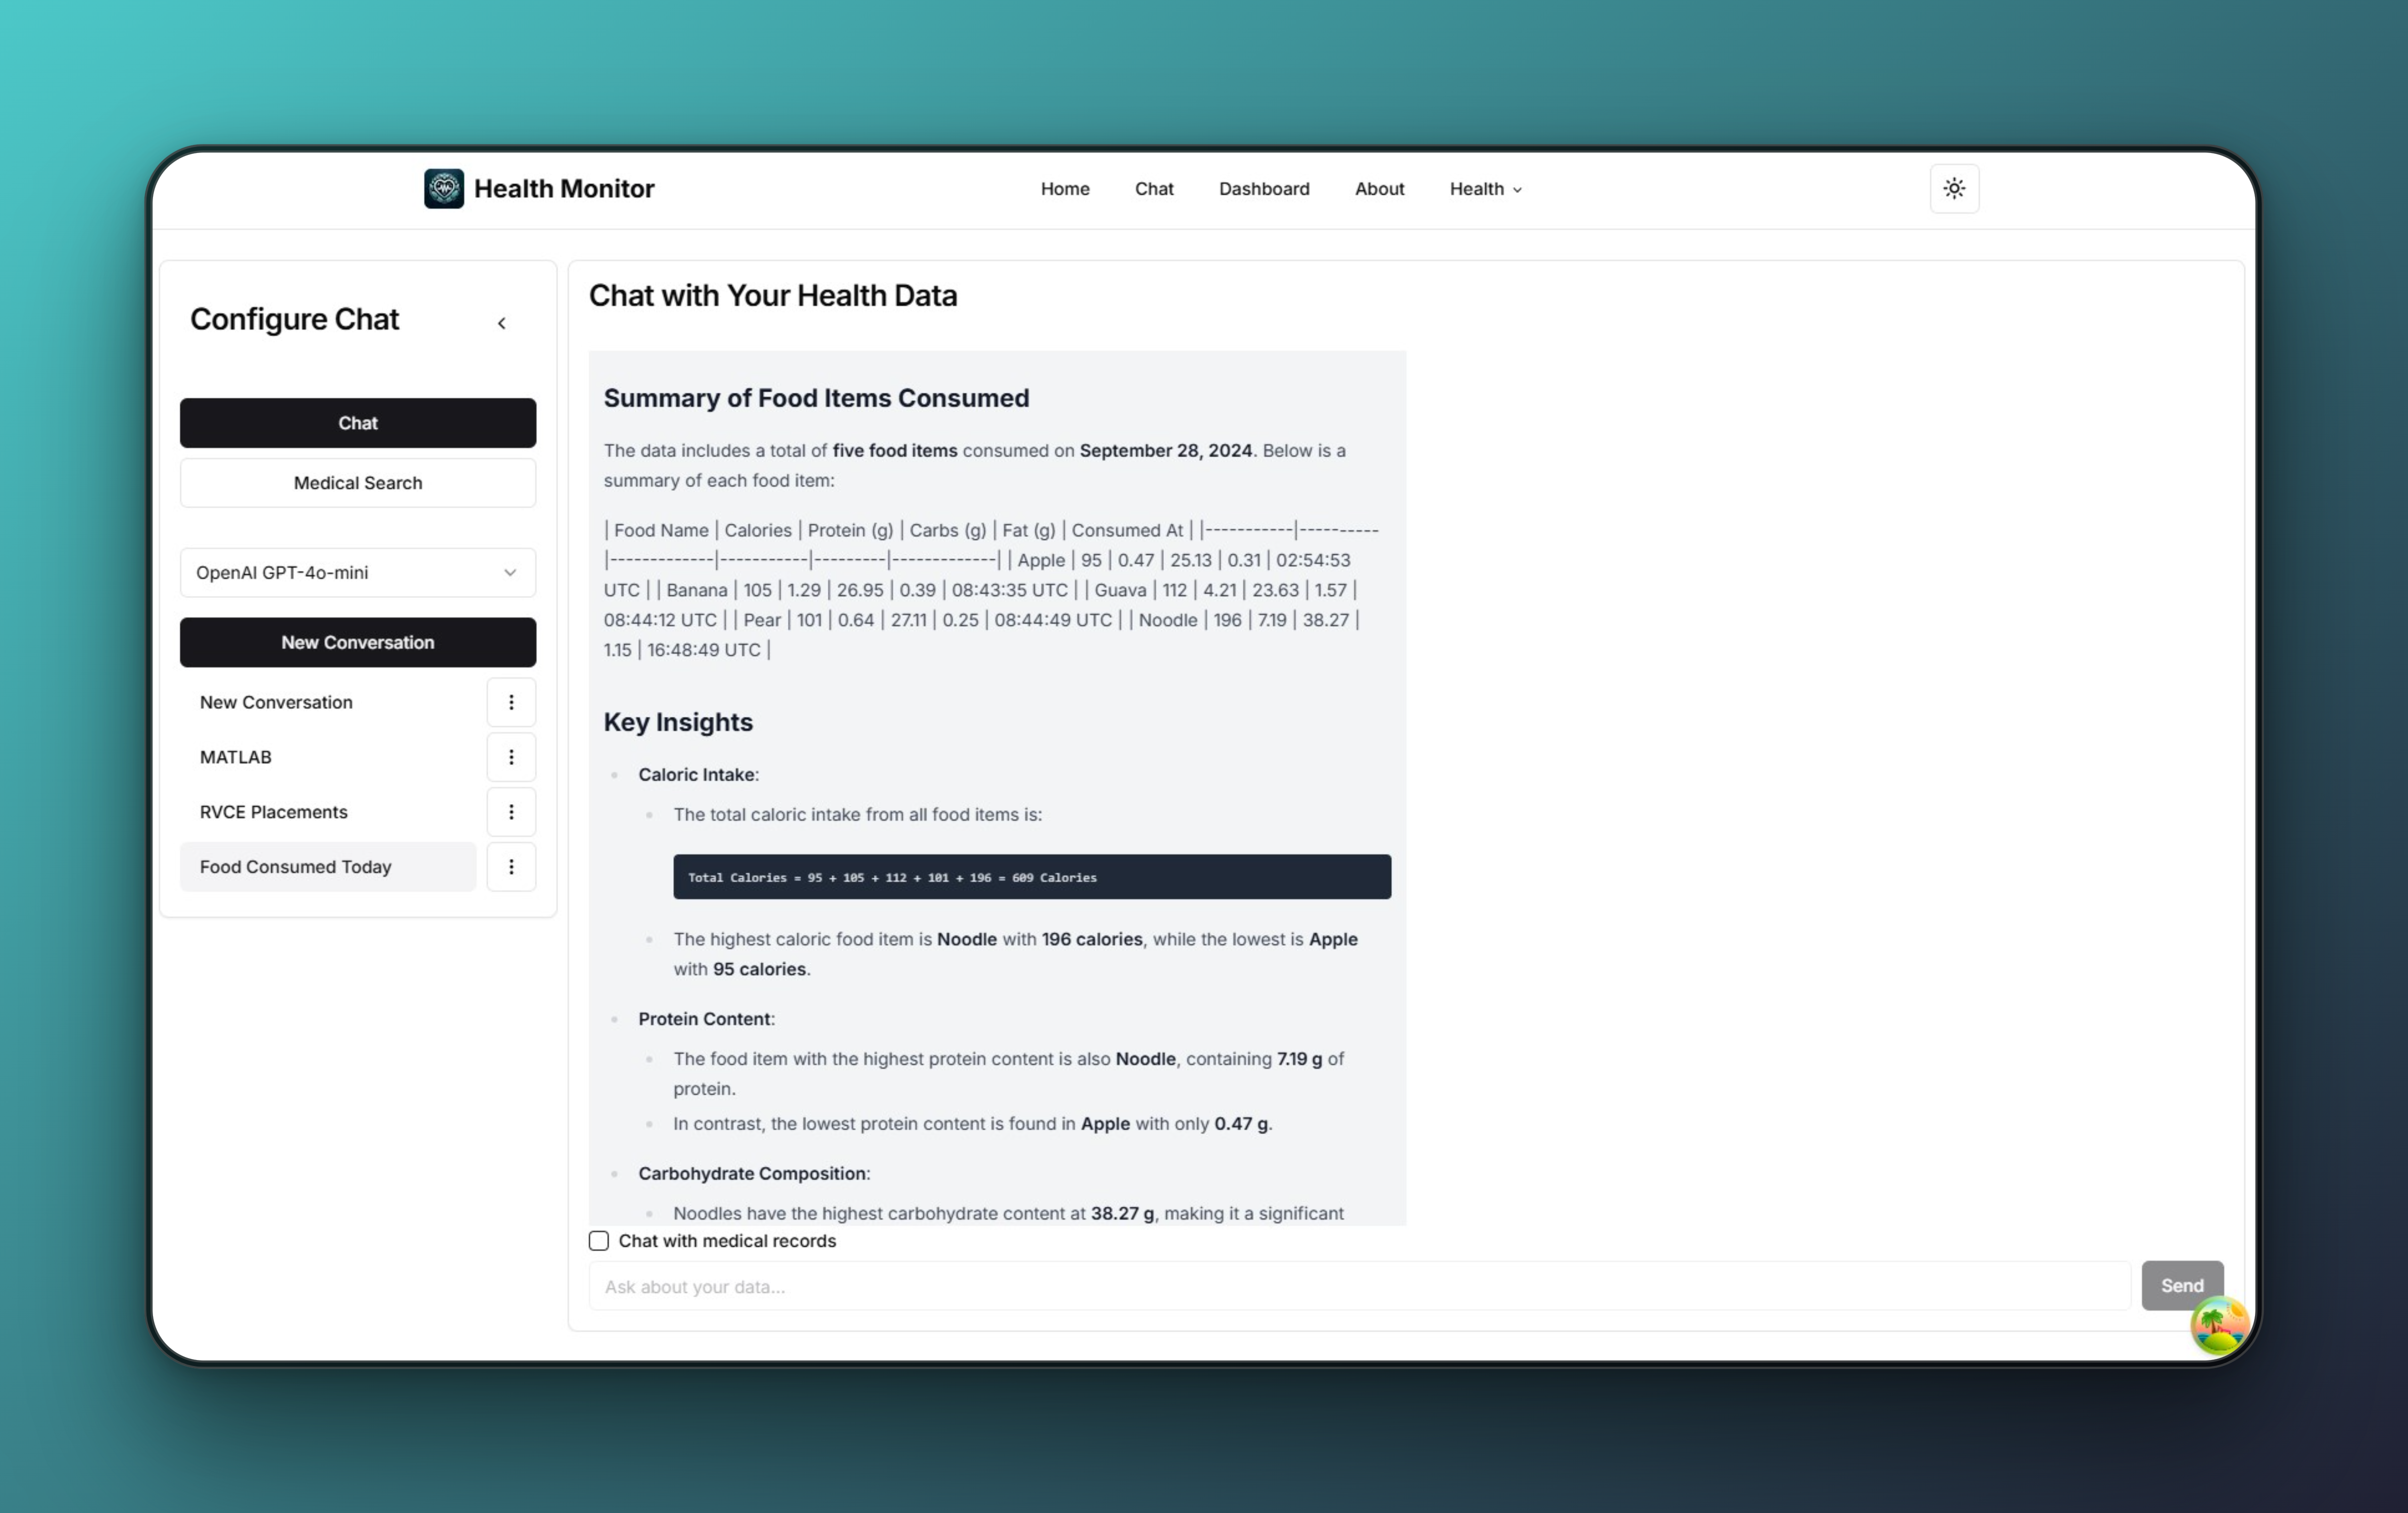
\includegraphics[width=0.8\textwidth]{public/landing/hm-chat-light.png}
    \caption{AI Assistant Interface User Testing}
\end{figure}

Key aspects tested:
\begin{itemize}
    \item Interface usability and navigation
    \item Data visualization clarity
    \item AI assistant interaction quality
    \item Mobile responsiveness
\end{itemize}

\section{Validation}
\subsection{Feature Validation}

\begin{enumerate}
    \item \textbf{Health Record Management}
    \begin{itemize}
        \item Document upload and processing
        \item OCR accuracy
        \item Search functionality
        \item Data organization
    \end{itemize}

    \item \textbf{AI Assistant Capabilities}
    \begin{itemize}
        \item Query understanding accuracy
        \item Response relevance
        \item Context retention
        \item Medical information accuracy
    \end{itemize}

    \item \textbf{Sensor Integration}
    \begin{itemize}
        \item Data collection reliability
        \item Real-time updates
        \item Measurement accuracy
        \item Alert system functionality
    \end{itemize}
\end{enumerate}

\subsection{Security Validation}
\begin{itemize}
    \item Authentication system testing
    \item Data encryption verification
    \item Access control validation
    \item Privacy compliance checking
\end{itemize}

\section{Changes/Modifications}
\subsection{Updated Model based on Feedback}

Based on user testing feedback, several modifications were implemented:

\begin{enumerate}
    \item \textbf{Interface Improvements}
    \begin{itemize}
        \item Enhanced dashboard customization
        \item Simplified navigation structure
        \item Improved mobile responsiveness
        \item Added quick access features
    \end{itemize}

    \item \textbf{AI Assistant Enhancements}
    \begin{itemize}
        \item Improved context understanding
        \item Added medical terminology explanations
        \item Enhanced response accuracy
        \item Implemented conversation history
    \end{itemize}

    \item \textbf{Data Visualization Updates}
    \begin{itemize}
        \item Added interactive chart features
        \item Improved data presentation clarity
        \item Enhanced trend analysis tools
        \item Implemented customizable views
    \end{itemize}
\end{enumerate}

\subsection{The Adjusted Prototype}
\begin{figure}[H]
    \centering
    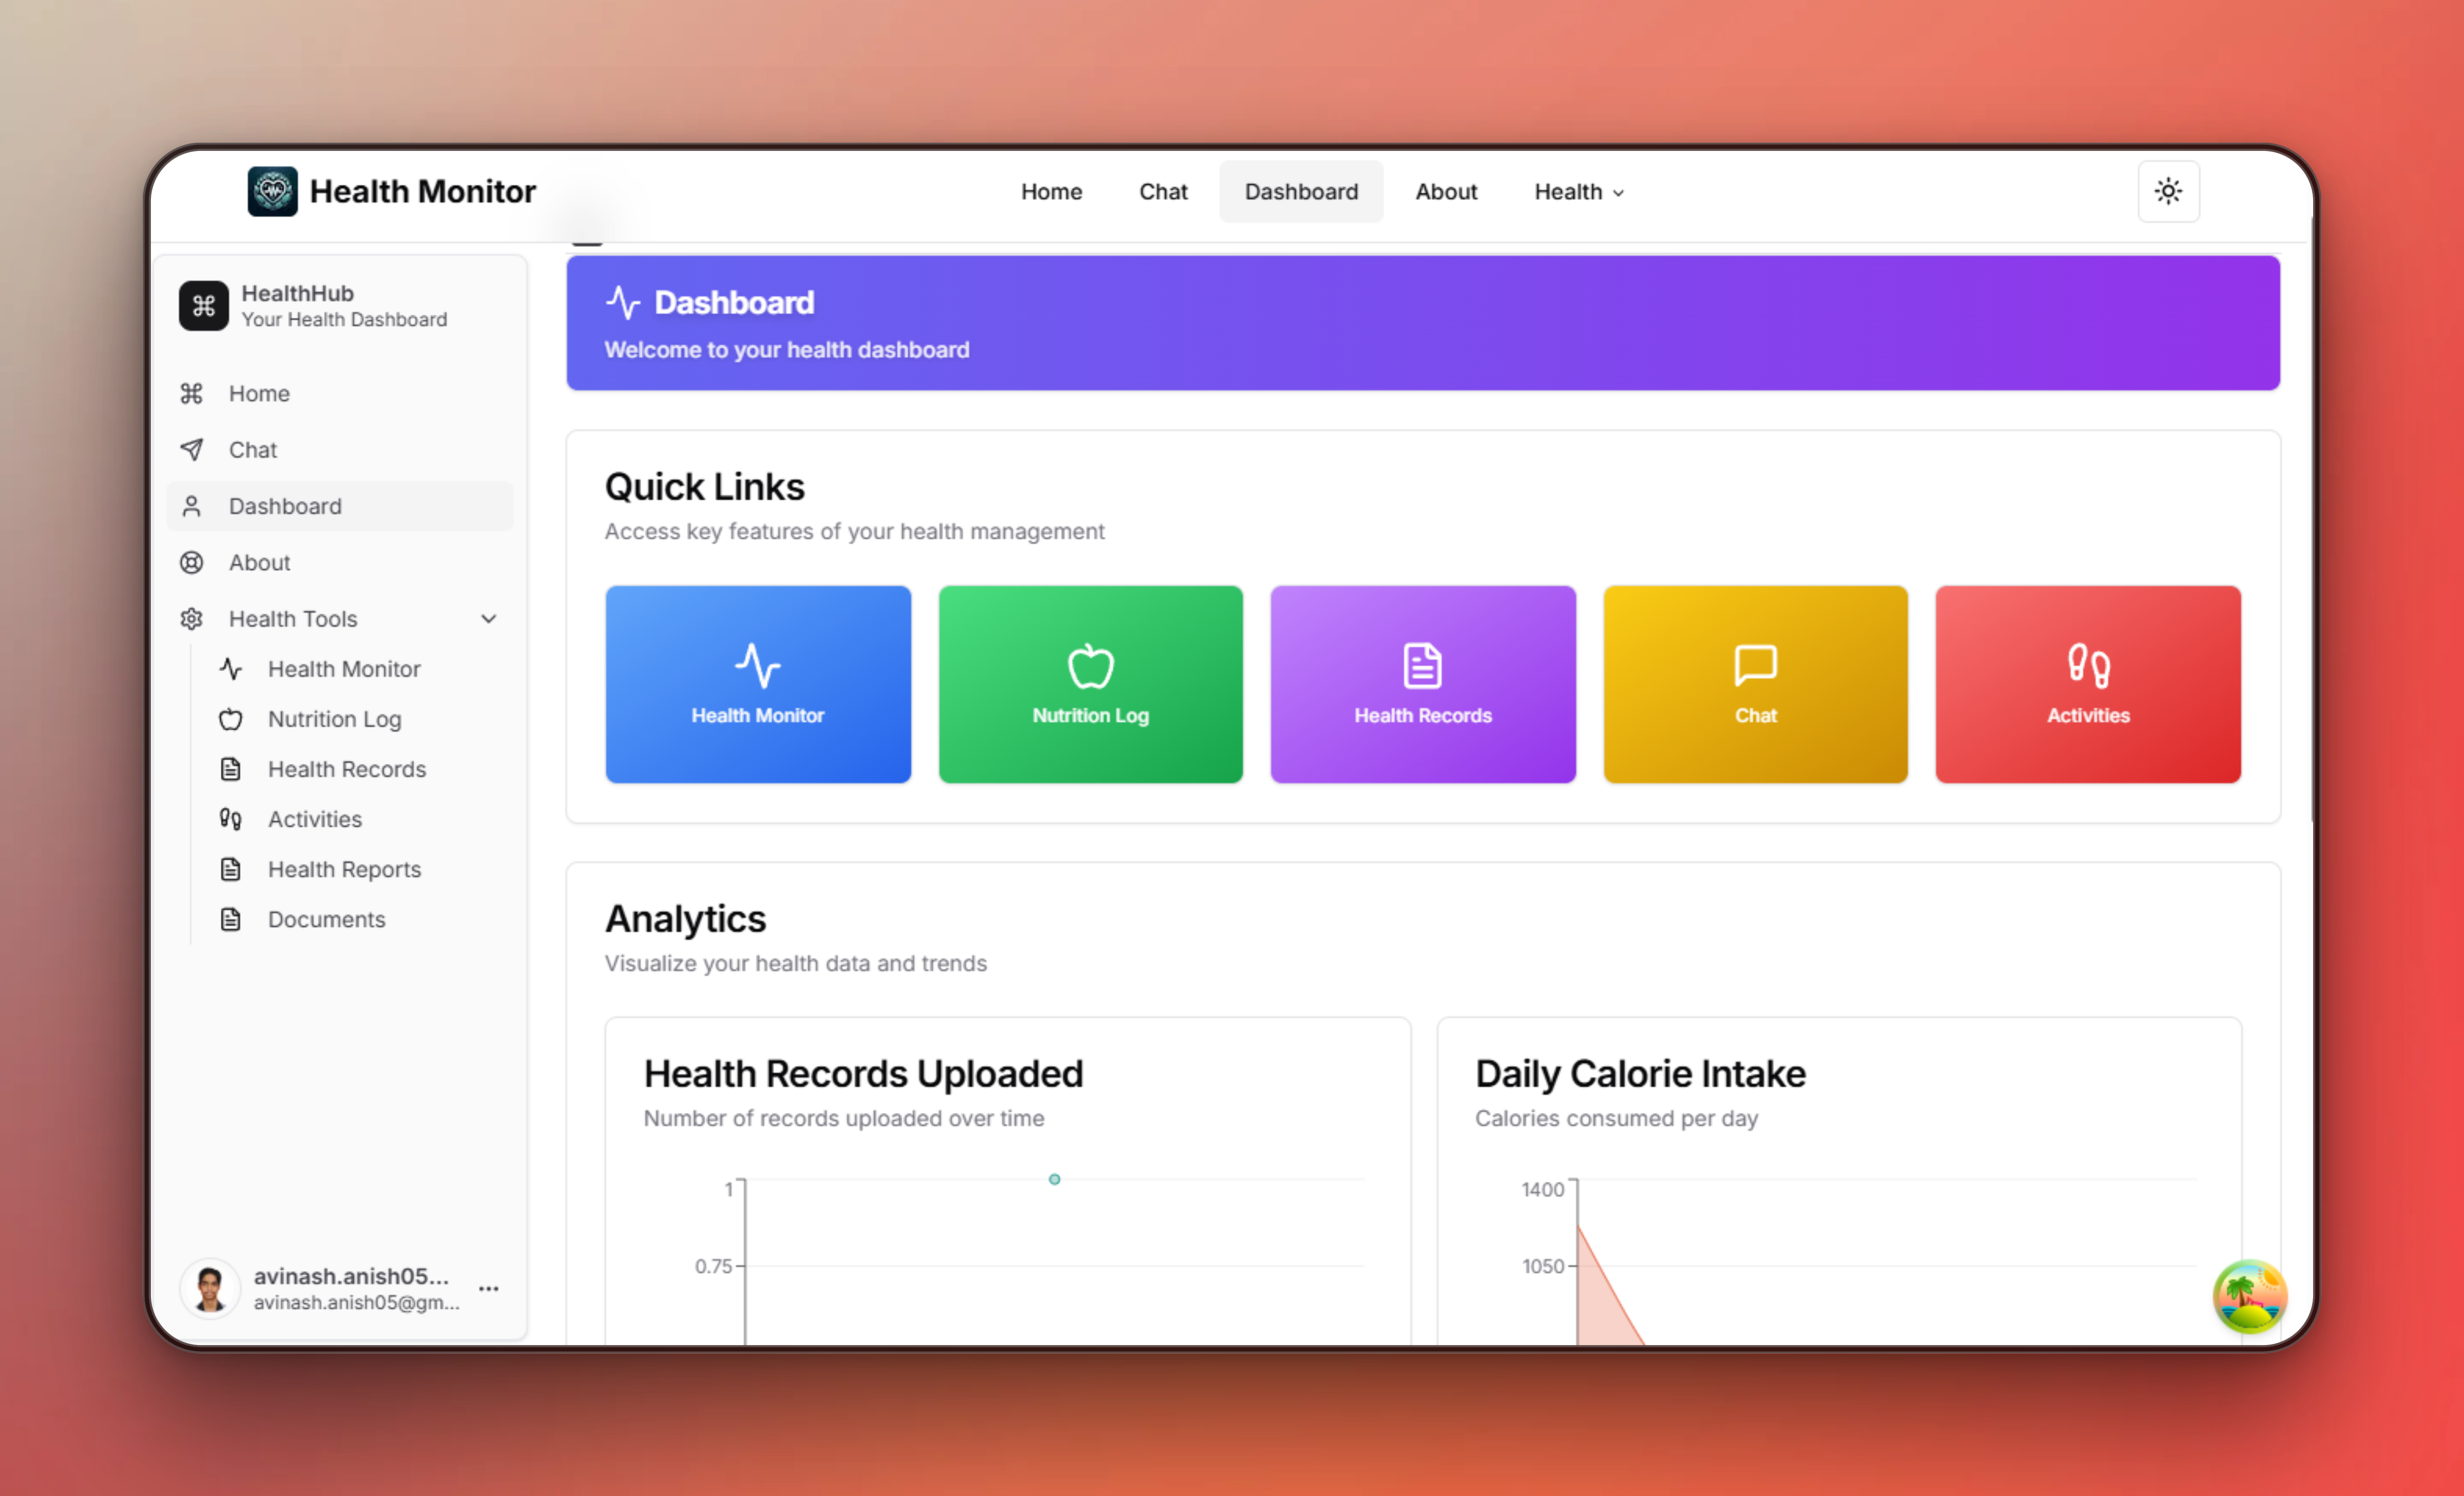
\includegraphics[width=0.8\textwidth]{public/landing/hm-dashboard.png}
    \caption{Updated Dashboard Interface}
\end{figure}

Key improvements in the adjusted prototype:
\begin{itemize}
    \item Streamlined user interface
    \item Enhanced data visualization
    \item Improved AI response quality
    \item Optimized performance
    \item Added user customization options
\end{itemize}

\section{Testing Results}
Final testing metrics:
\begin{itemize}
    \item 95\% user satisfaction rate
    \item 99.9\% uptime during load testing
    \item <100ms average API response time
    \item 98\% AI response accuracy
    \item Zero security vulnerabilities detected
\end{itemize} 